% see https://www.usenix.org/sites/default/files/template.la_.txt for original.
\documentclass[letterpaper,twocolumn,10pt]{article}
\usepackage{usenix,epsfig,endnotes}
\begin{document}

%don't want date printed
\date{}

%make title bold and 14 pt font (Latex default is non-bold, 16 pt)
\title{\Large \bf Federated Consistency for User-Centric Distributed Data Storage}

%for single author (just remove % characters)
\author{
{\rm Benjamin Bengfort}\\
University of Maryland\\
bengfort@cs.umd.edu
\and
{\rm Pete Keleher}\\
University of Maryland\\
keleher@cs.umd.edu
} % end author

\maketitle

% Use the following at camera-ready time to suppress page numbers.
% Comment it out when you first submit the paper for review.
% \thispagestyle{empty}


\subsection*{Abstract}

Federated consistency refers to a property of distributed systems wherein individual replicas maintain variable consistency levels. By allowing replicas to manage local storage independently of the system as a whole, a distributed storage system can take advantage of the high availability of eventually consistent systems while simultaneously providing strong guarantees about durability and ordering through a backbone consensus group. Unlike a homogenous, low latency data center, we believe that federated consistency enables heterogenous, variable latency, partition prone distributed storages such as those in personal clouds or in environments where backbone infrastructure has been lost and will perform better than centralized, high latency cloud storage.

\section{Introduction}

% I hate this paragraph: if we lead with the CAP theorem then no one will take the paper seriously. Particularly because of HAT and Brewer's article.

Distributed storage systems provide durability and availability by replicating data across multiple nodes, increasing redundancy and processor locality. These systems are described as a collective whole of independent, local nodes who share information over a potentially unstable or untimely network. As a result, most discussions concerning these types of systems focus on whether or not a node's view of the data is correct (consistency), whether or not clients can make progress (availability), and how the system repairs itself in the event of failure (partition tolerance).

Because of this characterization, the discussion of distributed storage systems is highly dependent on the network environment and distributed topology; and as a result, recent literature has shifted focus from networked file systems to cloud storages residing in data centers. In this environment, partitions are generally caused by wide area network failure, nodes are homogenous with similar capabilities, and intra-node network latency is minuscule relative to the client's connection. In such an environment, it is possible to reason about the trade-off between consistency and latency using a metric such as probabilistically bounded staleness \cite{bailis_quantifying_2014} and to explore a variety of consistency and transaction protocols from timing certainty using GPS and atomic clocks \cite{corbett_spanner_2013} to highly available key-value stores \cite{decandia_dynamo_2007}.

% Am I allowed to cite Dropbox?

By encapsulating these systems in a data center environment, performance measurements omit or treat as constant the bulk of latency encountered in real usage: the request latency from a user to the cloud and back again. In a user-oriented distributed data store such as Dropbox which syncs files across devices through a centralized cloud store it has been observed that frequent, short updates to user data causes inefficient traffic between the user's replicas and Dropbox \cite{li_efficient_2013} and that session acquisition is the primary bottleneck in synchronization performance \cite{drago_inside_2012}. Both of these studies propose a local middleware to alleviate these problems, but we take a stronger view: user devices should not simply be clients of web services that provide replication, they should be active participants acting as replicas themselves.

This forces us to have a new view of how systems behave. User devices have a variety of requirements and limitations from capacity to performance, and not all devices can perform leadership or relay roles. The distributed network is more partition prone as user devices are not always on or connected and mobility means highly variable latencies. Users switch devices, collaborate, and have preferences about what applications see what data and when. As a result, no single consistency, availability, or convergence mechanism can be directly applied.

In this paper we propose a vision for \textit{federated consistency}, an envelope term for a scheme where flexible consistency policies are mixed, modified, and coordinated to provide application-specific availability in user local networks. We present a base architecture for a distributed storage system that can utilize federated consistency but still provide strong guarantees, then discuss the consistency and consensus algorithms that might be implemented and how they interact. Finally, we propose a mechanism for evaluating the performance of such a system and highlight future work in this topic.

\subsection{Distributed Environment}

We assert that the computing and network environment of a distributed system plays a large role in determining not just the performance of the system, but in fact its behavior. A simple example is the election timeout parameter of the Raft consensus protocol, which must be significantly greater than the average time to broadcast and receive responses, and significantly less than the mean time between failure \cite{ongaro_search_2013}. If this requirement is not met, then the system will not be able to maintain a leader who will be displaced before heartbeat messages arrive or it will be unable to repair partitions in the quorum; the relationship of timeouts is dependent on the mean latency ($\lambda_{\mu}$) of the network. Extended studies on Raft propose heuristics such as $T = \lambda_{\mu} + 2\lambda_{\sigma}$ to determine timeouts based on the distribution of observed latencies, then setup the heartbeat as $\frac {T} {2}$ and an election timeout as the interval $U(T,2T)$ \cite{howard_raft_2015}. Real world systems such as etcd, a distributed key-value store by CoreOS, use a ``tick'' measure instead of milliseconds, which is computed in real time based on real performance; etcd recommends a 10:1 ratio of ticks for election timeouts to heartbeat messages \cite{mizerany_etcd_2016}.

% What about anti-entropy delays or other mechanisms?

Heuristics, distribution analysis, and modeling of the underlying distributed environment to determine system behavior are only effective when the environment exhibits a regular distribution of failure or latency. Such distributions are guaranteed in a data center where the environment is well managed and controlled. Most devices in a data center have similar specifications and are utilized for a similar suite of applications (servers or services that respond to requests). They are connected by high performance, low latency networks organized by switches in racks. These devices are always on, do not move, and have a number of amenities such as back up power and redundant disks.

In contrast, smaller scale, user-centric networks consist of fewer, application-specific devices that range from mobile devices to workstations. These devices connect to a variety of networks, from limited bandwidth cellular connections to high speed broadband links. A complete view of all devices for a single user will have irregular communication topologies based on location, e.g. a home network vs a work network, with mobile devices that can connect to both. Partitions can also easily occur when devices are powered off or leave the range of a network connection, and must be considered routine. Because a variety of applications with different data requirements or use cases are run on each device, a single consistency model (or view of the data) is not applicable. Moreover, the different specifications of each device mean that not all devices can equally participate in a distributed storage system (store a complete replica, participate as a leader, or act as a relay).

In order to reason about how a distributed system performs in a user centric context, we propose a model of the computing and network environment that has the following properties:

\begin{enumerate}
    \item \textbf{Heterogeneous devices}: there is a range in the performance and capacity of devices in the network, particularly in terms of storage capacity and the amount of time required to process and respond to messages.
    \item \textbf{Highly variable latencies}: network connections have a wide range of possible latencies, and the latency distribution also varies over time (for example as mobile devices move between networks).
    \item \textbf{Partition prone networks}: nodes become unreachable on a routine basis, and can rejoin the network at any time.
    \item \textbf{Irregular topologies}: not all nodes are connected at all times and moreover the topology is dynamic and connections can be added or removed.
\end{enumerate}

We believe that the challenge this environment poses to a distributed storage system will lead to valuable research both to address how consistency models that already exist operate in these environments as well as new protocols that increase performance or resilience. We also take the view that studying the more difficult case of these types of networks will also inform how more consistent environments behave.

\subsection{Requirements}

As the environment of distributed systems plays a large role in determining their behavior, so to does the specification or application of the system. Generally speaking the literature usually refers to file systems when discussing user centric distributed storage, and database systems for cloud storage, though the difference between the two can easily be blurred by representing a file system as a key-value store such as is done in the Amazon Simple Storage Service (S3) \cite{bermbach_eventual_2011}.

For the purposes of discussing federated consistency, we will generalize the requirements of the distributed system as follows. The system must manage multiple, independent objects whose data structure is defined solely within the context of the object (e.g. the system can be a simple key-value store, a relational database, or a file system). A single view of the system is given by a single user, and that view must be consistent with respect to the user's application. However, a system can maintain multiple views with multiple users interacting with the same objects (collaborative transactions).

Both in single and multi user contexts, the workload is variable with bursty accesses, unlike cloud storages which experience near constant workloads. This burstiness comes not only from routine work schedules but also because users typically don't access multiple devices simultaneously. Whereas many consistency models are designed for high availability through load balancing, the availability concerns in a user-centric distributed system tend to be application-specific. For example, photography workloads tend to be single writes (at the time of the photograph) but require multiple sequential reads as rapidly as possible. On the other hand, collaborative document editing requires linearizable, rapid writes along with read your write semantics.

The required guarantees for the system also are application specific. For the most part, durability is a constant and data loss is a bad thing. However, not all versions or temporary files need to be stored. Generally speaking more recent versions should remain durable, while historical versions can removed in a process called \textit{temporal aspect flattening}. Complete replication is also typically not a requirement, some devices require partial replication due to storage constraints, while others require only file formats specific to the application. Deciding what is stored on a partial replica is described as \textit{spatial aspect flattening}.  Finally, the rate at which objects are replicated is bound by the available bandwidth, some applications like video streaming should not share bandwidth through a replication process. Decisions about when and how replication occurs is referred to as \textit{synchronization aspect flattening}.

These requirements can be summarized as follows:

% Convert to a table
\begin{itemize}
    \item Management of multiple objects
    \item User centric views and multiple users
    \item Variable, bursty workloads
    \item Limited capacity and durability
    \item Partial replication
    \item Fair or limited resource use
    \item Multiple replicas and local replication
\end{itemize}

The last requirement dovetails with the irregular topologies discussed in the previous section. As the number of users in a distributed system increases, so do the number of replicas and partial replicas. Many consistency policies do not scale linearly therefore federated consistency needs to consider localities and partial quorums that emerge to global distributed semantics and guarantees.

\subsection{Examples}

We conclude the motivating section with three examples of distributed systems that might benefit from federated consistency: a personal cloud, disaster recovery/search and rescue, and highly mobile sensors.

\textbf{Personal Clouds} are a twist on distributed file systems that attempt to integrate storage across a wide area network and optionally with cloud storage. Personal clouds leverage mobile devices and high bandwidth connections to provide reliable replication. The primary advantage of a personal cloud is the low latency local network connections and the fact that synchronization to other devices does not require two round trips from a remote replica and back. Personal clouds put data ownership and management back into the user's hands who can better manage personal security and encryption as well as cost.

Single user personal clouds can be adapted into multiple user clouds with boundary-specific replication of shared objects. A hierarchical approach means that users can participate in multiple clouds or construct medium to large distributed storages. Collaboration and shared editing benefits from the same advantages, namely local network latency as opposed to multiple round trips to centralized application servers.

\textbf{Search and Rescue} networks are deployed in areas with no backbone connection either due to the remoteness of the activity or service interruptions after a disaster. As a result, these systems typically use mesh networking to create a local connectivity fabric, often in a hierarchical fashion. For example, in a large-scale disaster such as a hurricane, fire trucks may contain primary bandwidth links via satellite or point-to-point broadband connections, police squad cars may provide additional range by relaying wireless connections, and individual first responders may carry a variety of sensors and communication equipment. Remote units relay status information back to the primary bandwidth links, which in turn connect to a central operations command.

Due to the limited resources in such an environment and varying level of message priorities, multiple consistency levels are required. Routine updates with position information can be eventually consistent within some quality of service guarantee, however, alerts or triage information must arrive in a timely and correct fashion. Non-real-time data needs to be durable and ordered so that post operation analysis such as conducting structural audits or directing repair logistics is correct and verifiable.

\textbf{Highly Mobile Sensors} take advantage of new platforms such as robotic or arial vehicles to deploy a variety of sensors including audio and video to locations on demand. These sensors networks can be very large, such as video surveillance or photography (for example filmography recording a cycling race) or smaller and highly connective as in triage sensors in a hospital emergency room. Similar to search and rescue applications, these systems may have variable network connectivity or use mesh networking; however it is their mobility that is the key factor requiring federated consistency. Mobile sensors create irregular, dynamic topologies that require local consistency guarantees. Many strong consistency models require three phase commit for membership changes; but in a mobile sensor network, membership changes can be the norm not the exception. Federated consistency allows this type of distributed system to adapt as the topology adapts.

\section{Consistency Levels}

A federated consistency approach utilizes policies regarding temporal, spatial, and synchronization aspects to determine the behavior of a replica with regards to a set of objects. Consistency levels in such a system can be characterized on the range from eventually consistent to causal consistency to sequential consistency. This consistency range is also specified as the range between weak consistency (no node in the system is guaranteed to have the most up to date version) to strong consistency (all accesses view a single, consistent state).

\subsection{Eventual Consistency}

Eventual consistency is typically described using Werner Vogels' now popular definition: ``if no new updates are made to an object, eventually all accesses will return the last updated value'' \cite{vogels_eventually_2009}. This model offers liveness and availability to clients by simply returning the latest observed value of the object, however it is subject to staleness, in that the replica may be operating on old (stale) objects, though it can be shown that the extent of the staleness is bounded by the mean latency of the distributed system \cite{bailis_quantifying_2014,bailis_probabilistically_2012}.

Eventually consistent systems trade reduced response times for what is essentially a last-writer wins approach to data storage, which can have significant consequences for application behavior. Careful application design such as the use of commutative or associative operations on conflict-free replicated data types (CRDTs) \cite{shapiro_conflict-free_2011} or the careful application of immutable objects \cite{helland_immutability_2015} can mitigate some of the effects of this trade off. Other models such as Scatter employ multiple levels of consistency within the eventually consistent context, such as fully linearizable storage for a single key, but no linearization of multi-key transactions \cite{glendenning_scalable_2011}.

The implementation of eventually consistent systems utilizes anti-entropy \cite{demers_epidemic_1987} mechanisms to perform pairwise replication between two replica servers and to recover from partitions. For example, Bayou allows clients to perform file accesses locally then uses \cite{terry_managing_1995,terry_session_1994} anti-entropy sessions to propagate writes while also resolving conflicts through a policy based session guarantees. Bayou allows liveness, minimizes network usage, and delegates conflict handling to the application layer. Anti-entropy is introduced via gossip protocols (also called rumor mongering) where nodes spread rumors by randomly contacting a local neighbor and updating them. Gossip protocols solve the local broadcast problem which causes network flooding and are easily implemented in unstable networks with dynamic topologies \cite{haeupler_simple_2015}.

Recently, the Amazon Dynamo \cite{decandia_dynamo_2007} model has become the most popular reference application for eventually consistent systems, inspiring open source distributed data stores such as Apache Cassandra \cite{lakshman_cassandra_2010} and Project Voldemort \cite{feinberg2011project}. Dynamo combines well known techniques such as consistent hashing \cite{stoica_chord_2001}, object versioning using vector clocks \cite{lamport_time_1978}, partial quorums \cite{aiyer_availability_2005}, and gossip protocols to achieve a highly scalable, low latency key-value store. Unlike Bayou which relies on conflict resolution to maintain global consistency, Dynamo requires a configurable number of nodes to participate in read and write operations in a quorum-like fashion. Successful accesses therefore are guaranteed to be sequentially consistent among at least a majority of those N nodes, which can be used to repair conflicts using the vector timestamp of the access.

\subsection{Causal Consistency}

While the systems described wholly as eventually consistent in the previous section provide liveness, they do so by exposing data inconsistencies in response to client requests. As a result, weaker consistency models require mechanisms for conflict resolution and convergence that can be unnecessarily complex or simply farm the responsibility to the application layer. Causal consistency inherently strengthens the consistency model by requiring that objects that are causally related be ordered with respect to a read but still relaxes full linearizability by allowing partial ordering of unrelated objects    \cite{ahamad_causal_1990}.


COPS \cite{lloyd_dont_2011}

Bolt-On \cite{bailis_bolt-causal_2013}

Dangers of Causal, explicit solution \cite{bailis_potential_2012}

\subsection{Sequential Consistency}

Linearizability \cite{herlihy_linearizability_1990}

Happens Before \cite{lamport_time_1978}

Sequential Consistency \cite{attiya_sequential_1994}

Spanner \cite{corbett_spanner_2013}

\section{Consensus}

Paxos \cite{lamport_paxos_2001}

multi-paxos \cite{chandra_paxos_2007},

fast paxos \cite{lamport_fast_2006}

egalatarian paxos \cite{moraru_there_2013,moraru_egalitarian_2012}

raft \cite{ongaro_search_2013,howard_raft_2015}

stellar \cite{mazieres_stellar_2015}

warranties \cite{liu_warranties_2014}

\section{Federated Consistency}

\subsection{Interaction at Consistency Boundaries}

\subsubsection{Strong-Eventual}

\subsubsection{Strong-Causal}

\subsubsection{Eventual-Causal}

\subsection{Multiple Consistency Systems}

The integration of multiple consistency requires a strong consensus core in order to provide guarantees and manage conflicts, a scheme also used in Oceanstore \cite{kubiatowicz_oceanstore_2000} and \cite{gray_dangers_1996}.

\begin{figure}[h]
    \centering
    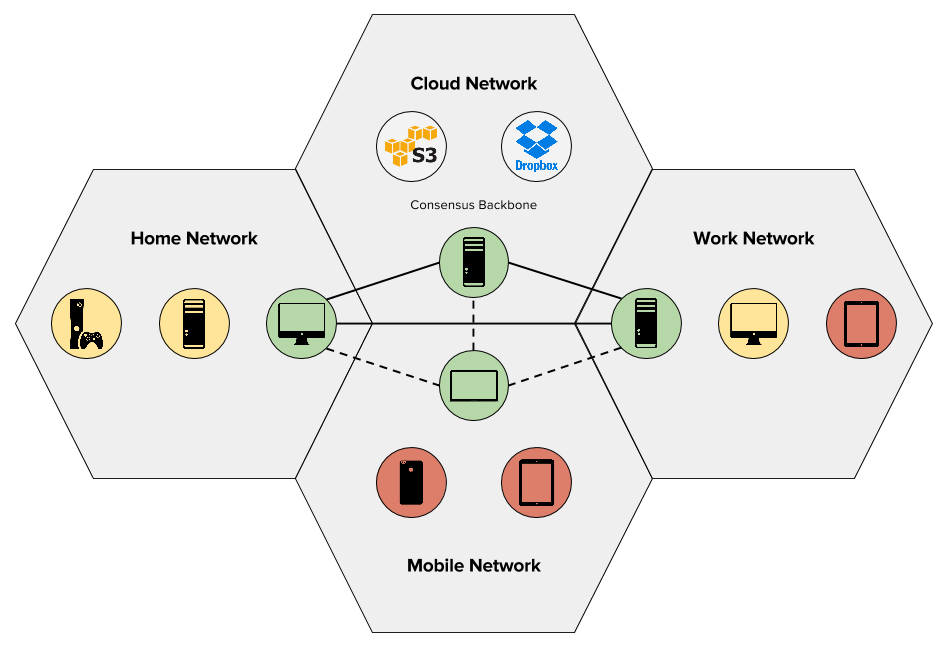
\includegraphics[width=0.5\textwidth]{figures/topology}
    \caption{The topology of a federated consistency model.}
\end{figure}

\begin{figure}[h]
    \centering
    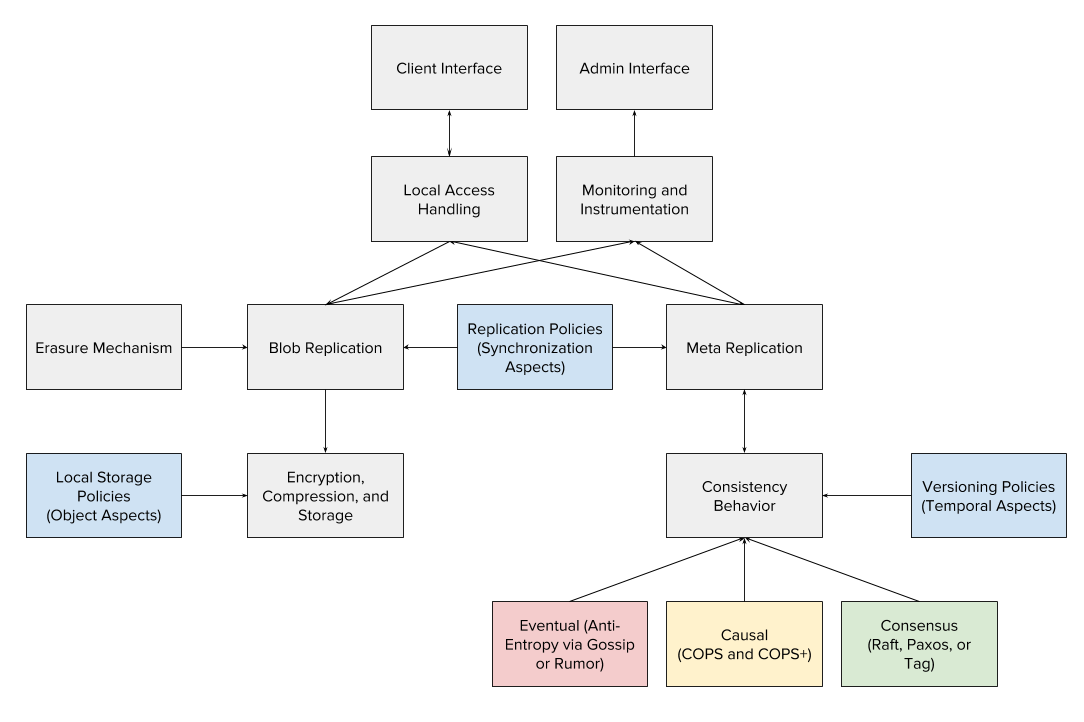
\includegraphics[width=0.5\textwidth]{figures/architecture}
    \caption{The component architecture of a federated consistency model.}
\end{figure}

\section{Experimental Discussion}

\begin{figure}[h]
    \centering
    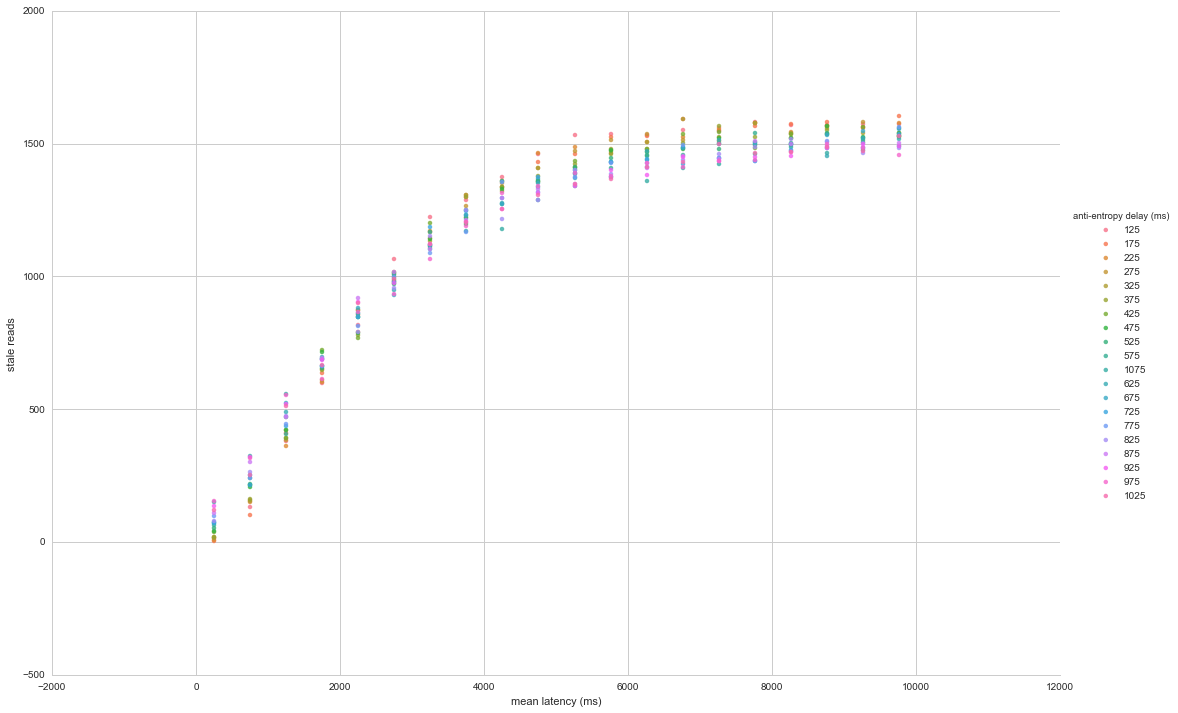
\includegraphics[width=0.5\textwidth]{figures/ae_stale_reads}
    \caption{Stale reads using eventual consistency with variable anti entropy delay.}
\end{figure}

\begin{figure}[h]
    \centering
    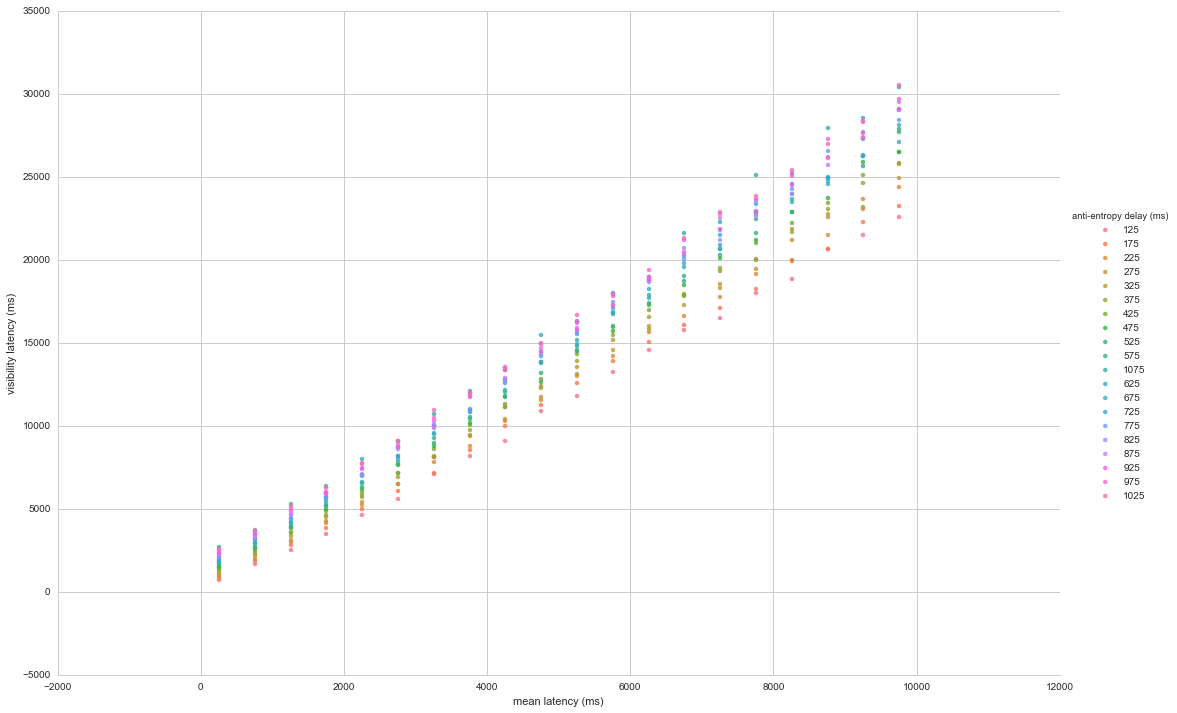
\includegraphics[width=0.5\textwidth]{figures/ae_viz_latency}
    \caption{Visibility latency using eventual consistency with variable anti entropy delay.}
\end{figure}

\begin{figure}[h]
    \centering
    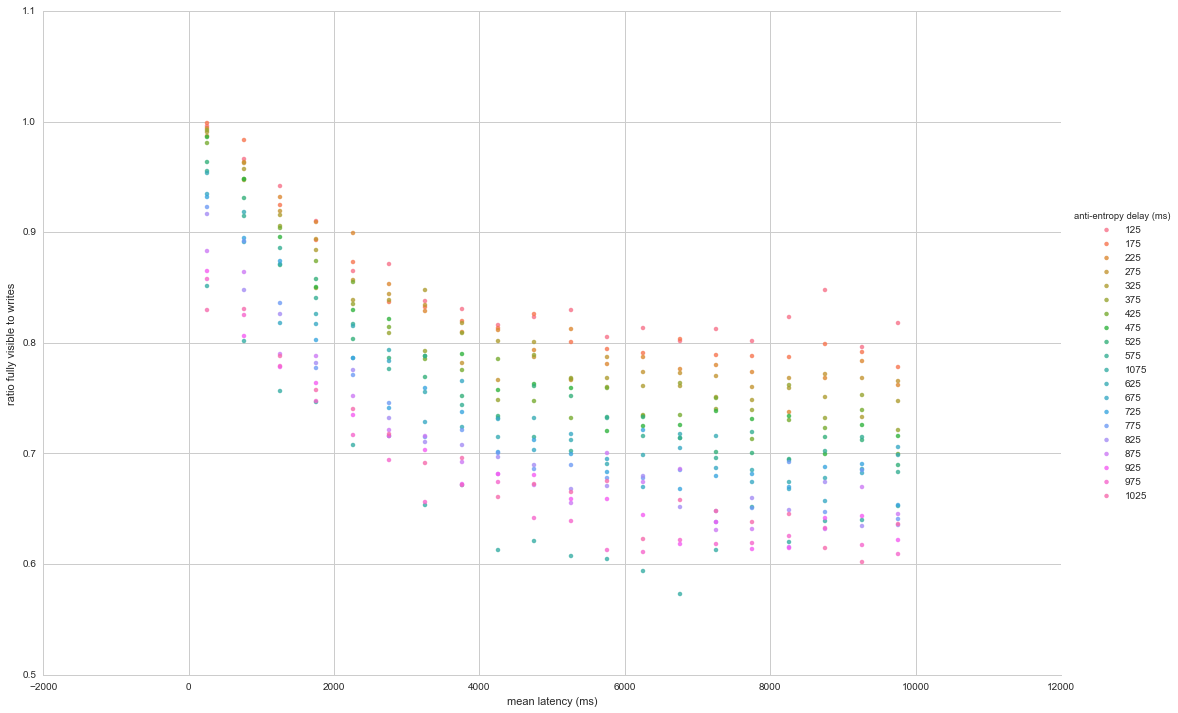
\includegraphics[width=0.5\textwidth]{figures/ae_viz_ratio}
    \caption{Ratio of fully visible writes to total writes using eventual consistency with variable anti entropy delay.}
\end{figure}

\begin{figure}[h]
    \centering
    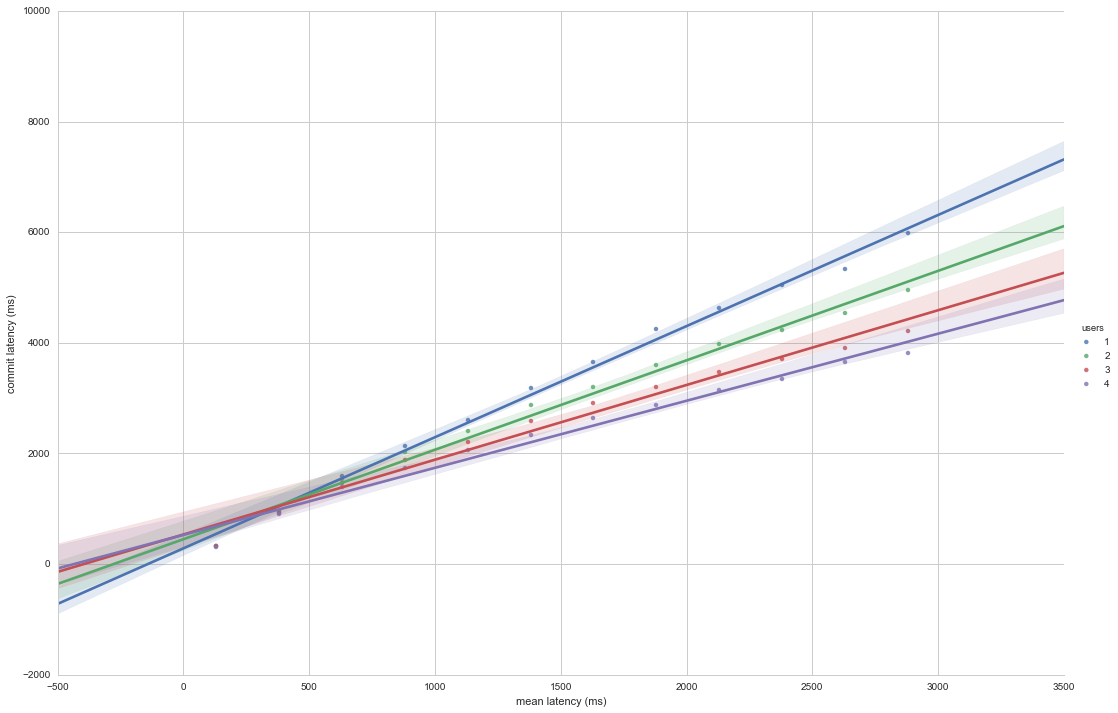
\includegraphics[width=0.5\textwidth]{figures/raft_commit_latency}
    \caption{Commit latency in Raft with increasing numbers of users.}
\end{figure}

\section{Conclusion}

\section*{Acknowledgments}

{\footnotesize \bibliographystyle{acm}
\bibliography{references}}

% uncomment to include end notes.
% \theendnotes

\end{document}
